% Options for packages loaded elsewhere
\PassOptionsToPackage{unicode}{hyperref}
\PassOptionsToPackage{hyphens}{url}
%
\documentclass[
  oneside]{book}
\usepackage{amsmath,amssymb}
\usepackage{lmodern}
\usepackage{iftex}
\ifPDFTeX
  \usepackage[T1]{fontenc}
  \usepackage[utf8]{inputenc}
  \usepackage{textcomp} % provide euro and other symbols
\else % if luatex or xetex
  \usepackage{unicode-math}
  \defaultfontfeatures{Scale=MatchLowercase}
  \defaultfontfeatures[\rmfamily]{Ligatures=TeX,Scale=1}
\fi
% Use upquote if available, for straight quotes in verbatim environments
\IfFileExists{upquote.sty}{\usepackage{upquote}}{}
\IfFileExists{microtype.sty}{% use microtype if available
  \usepackage[]{microtype}
  \UseMicrotypeSet[protrusion]{basicmath} % disable protrusion for tt fonts
}{}
\makeatletter
\@ifundefined{KOMAClassName}{% if non-KOMA class
  \IfFileExists{parskip.sty}{%
    \usepackage{parskip}
  }{% else
    \setlength{\parindent}{0pt}
    \setlength{\parskip}{6pt plus 2pt minus 1pt}}
}{% if KOMA class
  \KOMAoptions{parskip=half}}
\makeatother
\usepackage{xcolor}
\IfFileExists{xurl.sty}{\usepackage{xurl}}{} % add URL line breaks if available
\IfFileExists{bookmark.sty}{\usepackage{bookmark}}{\usepackage{hyperref}}
\hypersetup{
  pdftitle={Data Science \& Machine Learning},
  pdfauthor={Dieter Greipl},
  hidelinks,
  pdfcreator={LaTeX via pandoc}}
\urlstyle{same} % disable monospaced font for URLs
\usepackage{color}
\usepackage{fancyvrb}
\newcommand{\VerbBar}{|}
\newcommand{\VERB}{\Verb[commandchars=\\\{\}]}
\DefineVerbatimEnvironment{Highlighting}{Verbatim}{commandchars=\\\{\}}
% Add ',fontsize=\small' for more characters per line
\usepackage{framed}
\definecolor{shadecolor}{RGB}{248,248,248}
\newenvironment{Shaded}{\begin{snugshade}}{\end{snugshade}}
\newcommand{\AlertTok}[1]{\textcolor[rgb]{0.94,0.16,0.16}{#1}}
\newcommand{\AnnotationTok}[1]{\textcolor[rgb]{0.56,0.35,0.01}{\textbf{\textit{#1}}}}
\newcommand{\AttributeTok}[1]{\textcolor[rgb]{0.77,0.63,0.00}{#1}}
\newcommand{\BaseNTok}[1]{\textcolor[rgb]{0.00,0.00,0.81}{#1}}
\newcommand{\BuiltInTok}[1]{#1}
\newcommand{\CharTok}[1]{\textcolor[rgb]{0.31,0.60,0.02}{#1}}
\newcommand{\CommentTok}[1]{\textcolor[rgb]{0.56,0.35,0.01}{\textit{#1}}}
\newcommand{\CommentVarTok}[1]{\textcolor[rgb]{0.56,0.35,0.01}{\textbf{\textit{#1}}}}
\newcommand{\ConstantTok}[1]{\textcolor[rgb]{0.00,0.00,0.00}{#1}}
\newcommand{\ControlFlowTok}[1]{\textcolor[rgb]{0.13,0.29,0.53}{\textbf{#1}}}
\newcommand{\DataTypeTok}[1]{\textcolor[rgb]{0.13,0.29,0.53}{#1}}
\newcommand{\DecValTok}[1]{\textcolor[rgb]{0.00,0.00,0.81}{#1}}
\newcommand{\DocumentationTok}[1]{\textcolor[rgb]{0.56,0.35,0.01}{\textbf{\textit{#1}}}}
\newcommand{\ErrorTok}[1]{\textcolor[rgb]{0.64,0.00,0.00}{\textbf{#1}}}
\newcommand{\ExtensionTok}[1]{#1}
\newcommand{\FloatTok}[1]{\textcolor[rgb]{0.00,0.00,0.81}{#1}}
\newcommand{\FunctionTok}[1]{\textcolor[rgb]{0.00,0.00,0.00}{#1}}
\newcommand{\ImportTok}[1]{#1}
\newcommand{\InformationTok}[1]{\textcolor[rgb]{0.56,0.35,0.01}{\textbf{\textit{#1}}}}
\newcommand{\KeywordTok}[1]{\textcolor[rgb]{0.13,0.29,0.53}{\textbf{#1}}}
\newcommand{\NormalTok}[1]{#1}
\newcommand{\OperatorTok}[1]{\textcolor[rgb]{0.81,0.36,0.00}{\textbf{#1}}}
\newcommand{\OtherTok}[1]{\textcolor[rgb]{0.56,0.35,0.01}{#1}}
\newcommand{\PreprocessorTok}[1]{\textcolor[rgb]{0.56,0.35,0.01}{\textit{#1}}}
\newcommand{\RegionMarkerTok}[1]{#1}
\newcommand{\SpecialCharTok}[1]{\textcolor[rgb]{0.00,0.00,0.00}{#1}}
\newcommand{\SpecialStringTok}[1]{\textcolor[rgb]{0.31,0.60,0.02}{#1}}
\newcommand{\StringTok}[1]{\textcolor[rgb]{0.31,0.60,0.02}{#1}}
\newcommand{\VariableTok}[1]{\textcolor[rgb]{0.00,0.00,0.00}{#1}}
\newcommand{\VerbatimStringTok}[1]{\textcolor[rgb]{0.31,0.60,0.02}{#1}}
\newcommand{\WarningTok}[1]{\textcolor[rgb]{0.56,0.35,0.01}{\textbf{\textit{#1}}}}
\usepackage{longtable,booktabs,array}
\usepackage{calc} % for calculating minipage widths
% Correct order of tables after \paragraph or \subparagraph
\usepackage{etoolbox}
\makeatletter
\patchcmd\longtable{\par}{\if@noskipsec\mbox{}\fi\par}{}{}
\makeatother
% Allow footnotes in longtable head/foot
\IfFileExists{footnotehyper.sty}{\usepackage{footnotehyper}}{\usepackage{footnote}}
\makesavenoteenv{longtable}
\usepackage{graphicx}
\makeatletter
\def\maxwidth{\ifdim\Gin@nat@width>\linewidth\linewidth\else\Gin@nat@width\fi}
\def\maxheight{\ifdim\Gin@nat@height>\textheight\textheight\else\Gin@nat@height\fi}
\makeatother
% Scale images if necessary, so that they will not overflow the page
% margins by default, and it is still possible to overwrite the defaults
% using explicit options in \includegraphics[width, height, ...]{}
\setkeys{Gin}{width=\maxwidth,height=\maxheight,keepaspectratio}
% Set default figure placement to htbp
\makeatletter
\def\fps@figure{htbp}
\makeatother
\setlength{\emergencystretch}{3em} % prevent overfull lines
\providecommand{\tightlist}{%
  \setlength{\itemsep}{0pt}\setlength{\parskip}{0pt}}
\setcounter{secnumdepth}{5}

%\usepackage{booktabs}
%\usepackage{longtable}
%\usepackage[bf,singlelinecheck=off]{caption}

%\usepackage{Alegreya}
%\usepackage[scale=.8]{sourcecodepro}

%\usepackage[a4paper, top=1cm, bottom=1cm ]{geometry}
%\geometry{a4paper,hmargin={2cm,1.5cm},}
\usepackage[a4paper,hmargin={2cm,1.5cm}, vmargin={1.5cm,1.5cm} ]{geometry}
\usepackage[rigidchapters]{titlesec}

%---------------------------------- Seitenlayout
\textwidth 160mm
\textheight 240mm
\topmargin=-15mm

\setlength\oddsidemargin{(\paperwidth-\textwidth)/2 - 1in}
\setlength\topmargin{(\paperheight-\textheight
-\headheight-\headsep-\footskip)/2 - 1in}

\setcounter{secnumdepth}{2}
\setcounter{tocdepth}{2}


% Kopfzeile unterstreichen
\usepackage[
headsepline,
%footsepline % no separation line for page number
]{scrlayer-scrpage}

\titlespacing{\subsection}{0pt}{3ex}{-0.5ex}
\titlespacing{\subsubsection}{0pt}{2ex}{-0.5ex}

\setlength{\parindent}{1em}
\usepackage{graphicx}

% Turn off autmatic crearion of the coverpage
\let\oldmaketitle\maketitle
\AtBeginDocument{\let\maketitle\relax}

%Zim Testen
\usepackage{blindtext}

\usepackage{color}



\ifLuaTeX
  \usepackage{selnolig}  % disable illegal ligatures
\fi
\usepackage[]{natbib}
\bibliographystyle{apalike}

\title{Data Science \& Machine Learning}
\author{Dieter Greipl}
\date{2022-02-01}

\begin{document}
\maketitle


\begin{titlepage}

\begin{center}

\Huge \textbf{Data Science und Machine Learning}

\Large \textbf{Einführung für Studierende der Betriebswirtschaftslehre und Wirtschaftsinformatik}


\end{center}

\noindent\makebox[\textwidth][c]{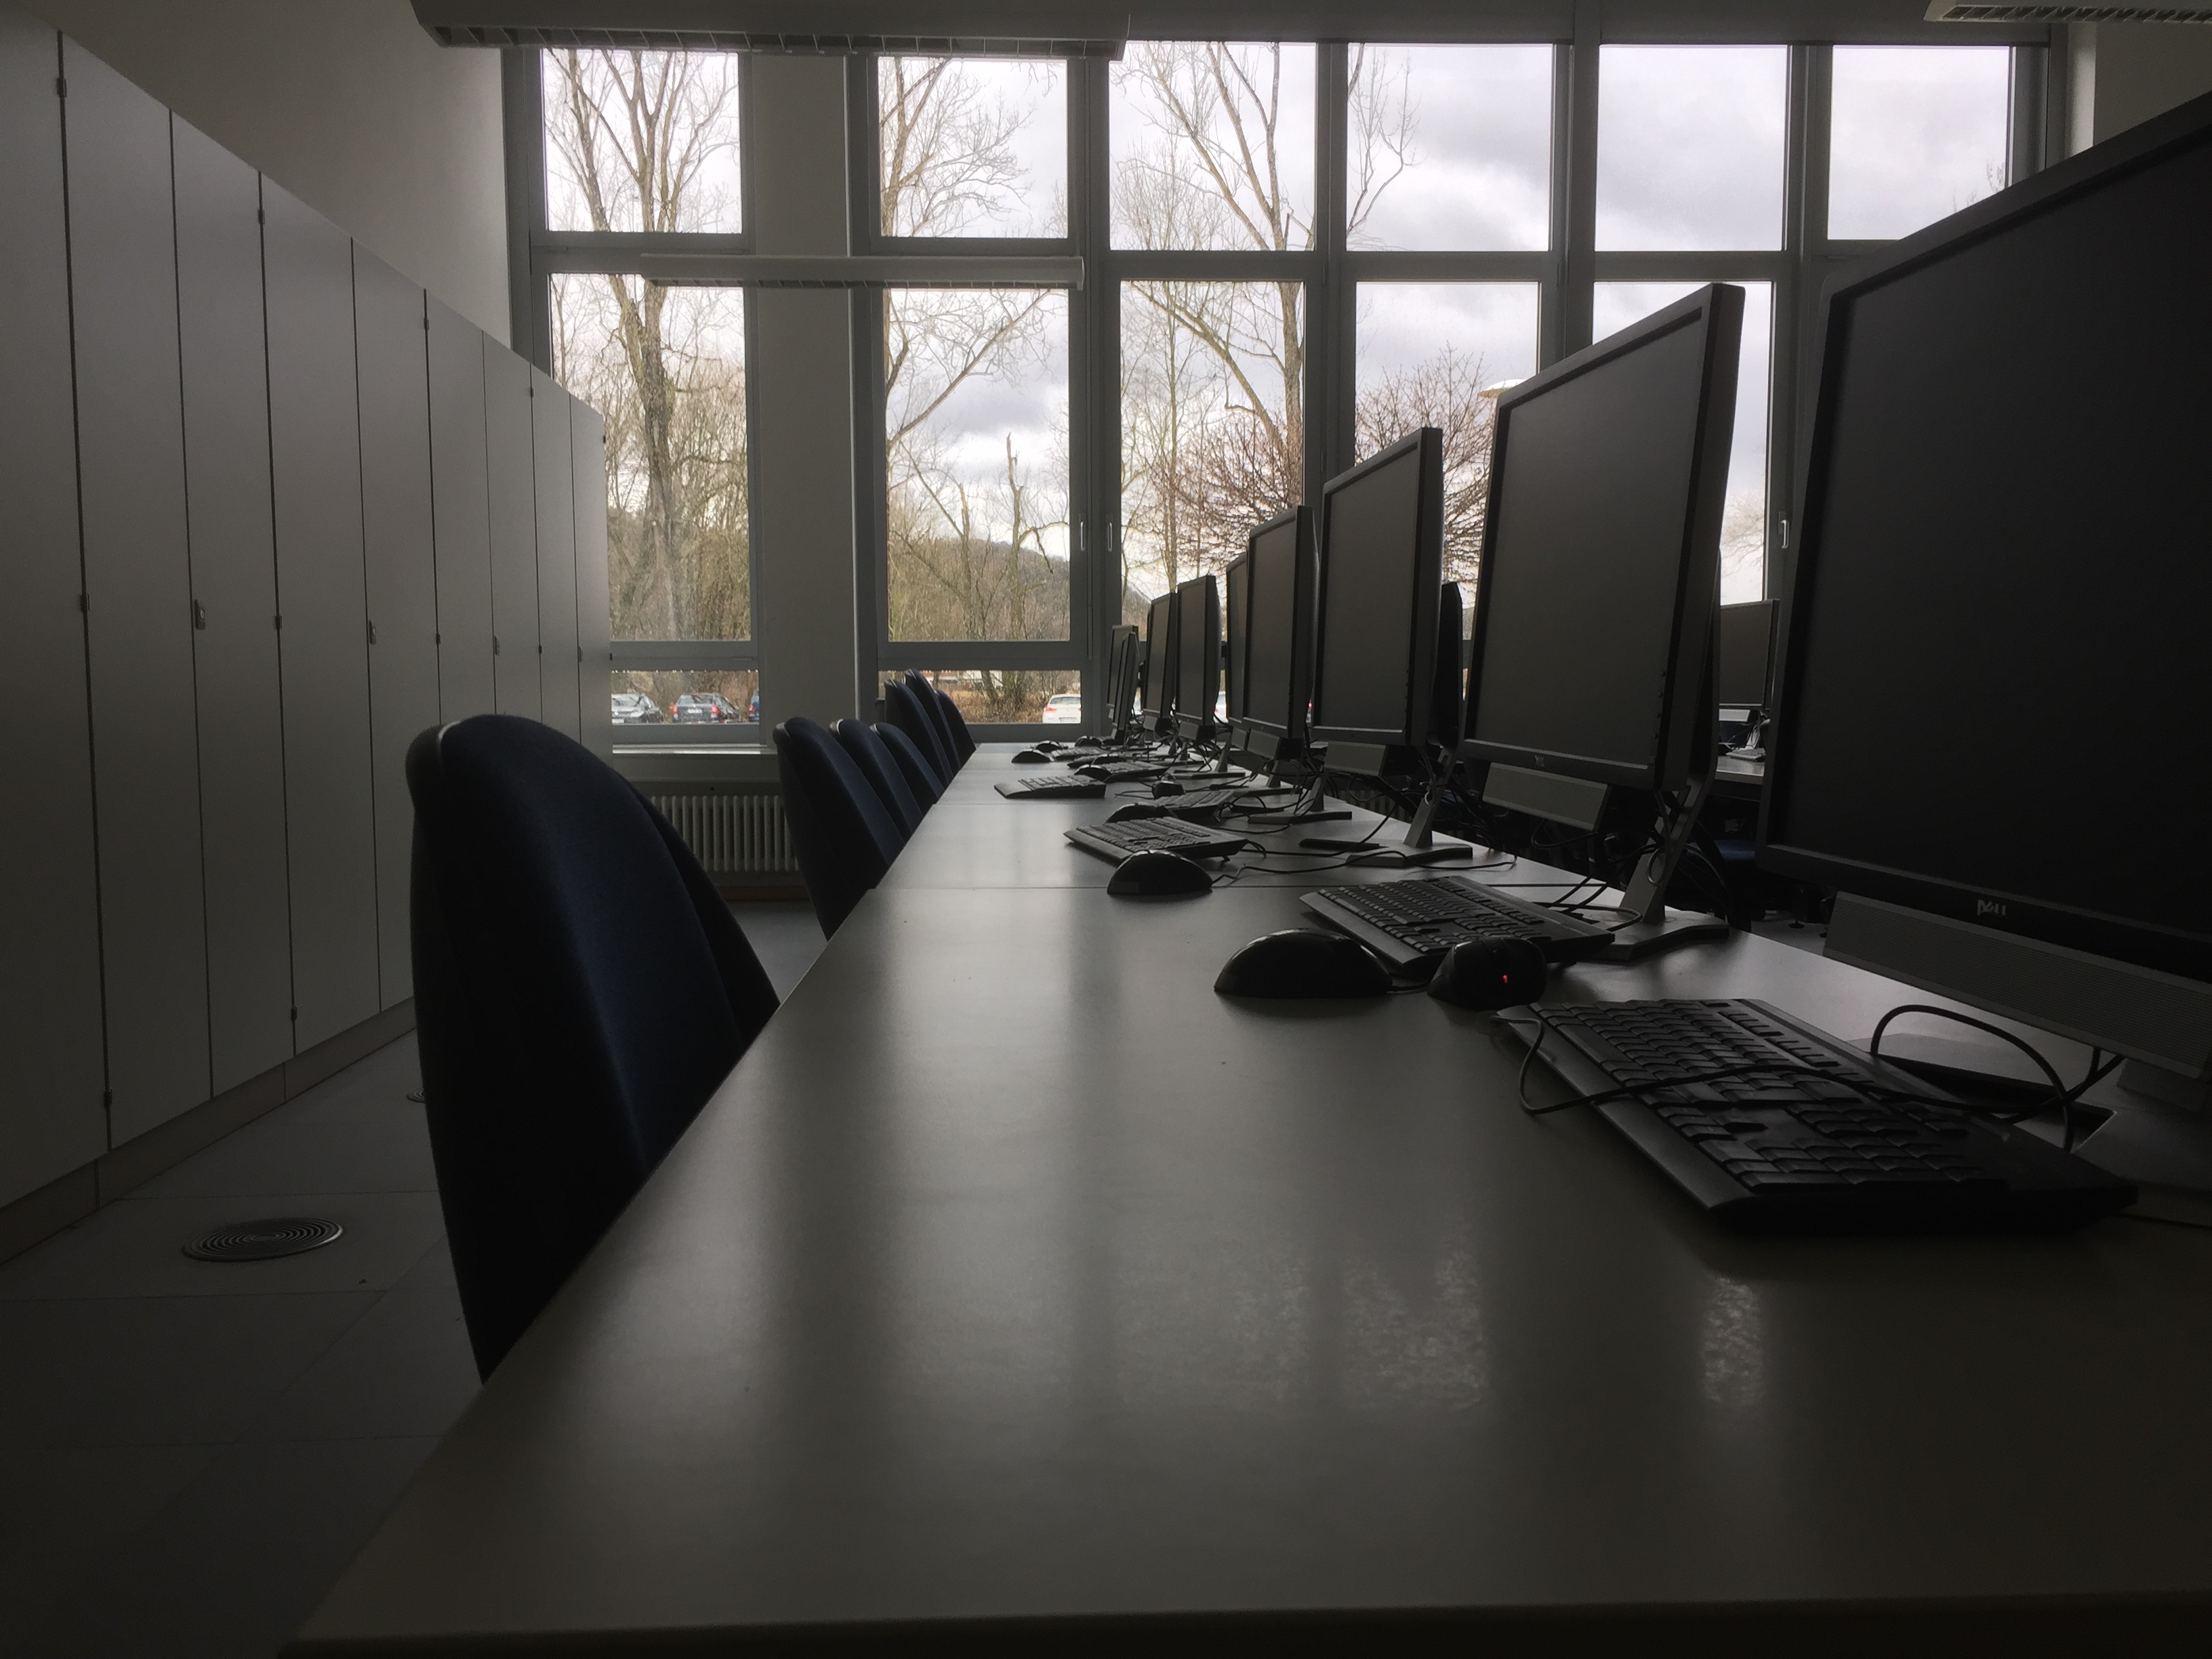
\includegraphics[width=\paperwidth]{assets/cover_1.jpg}}

%textbox unten rechts
\vspace{-3cm}
\hfill
\begin{minipage}[b][1cm][t]{10cm}
  \color{white}
  \begin{flushright}
     \Huge\textbf{Dieter Greipl}\\
     \Large\textbf{Hochschule Landshut}\\
  \end{flushright}
\end{minipage}

\end{titlepage}

% Zweite Seite ---------------------------------------
\begin{titlepage}
\hfill
\begin{minipage}[r][10cm][t]{10cm}
\large \textbf{Danke}\\
	Dieses Buch entstand im Sommersemester 2022. Vielen Dank an meine Sudierenden für zahlreiche Hinweise.
\end{minipage}

\vfill
%textbox unten rechts
\begin{minipage}[b][10cm][b]{10cm}
\large{Copyright}\\
	...
\end{minipage}

\end{titlepage}



{
\setcounter{tocdepth}{1}
\tableofcontents
}
\hypertarget{willkommen}{%
\chapter*{Willkommen}\label{willkommen}}
\addcontentsline{toc}{chapter}{Willkommen}

Dieses Skript entstand (und entsteht) aus meinen Lehrveranstaltungen rund um das Thema \textbf{Data Science \& Machine Learning}. Die Inhalte richten sich an Studierende, die erste Schritte auf das KI -Spielfeld wagen und das Potential von datengetriebenen Lösungsverfahren verstehen wollen.

Insofern richtet sich die Darstellung an Studierende mit vertieftem Interesse an KI, die einen für Studierende angemessenes Vorwissen im Bereich Mathematik mitbringen. Vorkenntnisse im Bereich der Programmierung sind nicht nötig, aber natürlich hilfreich.

Ich habe mich bemüht, zahlreiche Übungsbeispiele und Youtube-Videos einzubauen. Viele Themen lassen sich so besser darstellen. Sofern es Medien im Netz gibt, die die Sachverhalte gut darstellen, werde ich entsprechenden Links einbauen. Der Autor muss ja nicht der Meinung sein, alles besser zu können. Gleichwohl darf dadurch der rote Faden nicht verloren gehen.

\hypertarget{vorbereitungen}{%
\section{Vorbereitungen}\label{vorbereitungen}}

Dieses Skript ist als Unterlage für zahlreichen praktische Übungen mit Python angelegt. Ich werde hierzu \href{https://colab.research.google.com/}{\textbf{Colab-Notebooks}} verwenden. Sie brauchen hierzu ein \textbf{Google-Konto}.

Noch einige Hinweise an Studierende meiner Module:

\begin{itemize}
\tightlist
\item
  Die folgende Youtube-Playlist kann zur Vertiefung einzelner Stoffteile nutzen: \href{https://youtube.com/playlist?list=PLfGN40VwjduJPvtP9QUjC0rjM6-ePT9bg}{Youtube Playlist}
\item
  Wenige Passagen in diesem Skript sind eventuell in englischer Sprache gehalten.
\item
  Dieses Skript

  \begin{itemize}
  \tightlist
  \item
    befindet sich in Teilen im Aufbau, leichte Fehler sind also möglich (und wahrscheinlich - für Hinweise bin ich dankbar)
  \item
    geht nach der Prüfung off-line
  \end{itemize}
\end{itemize}

\hypertarget{python---quickstart}{%
\chapter{Python - Quickstart}\label{python---quickstart}}

\hypertarget{colab-notebooks}{%
\section{Colab-Notebooks}\label{colab-notebooks}}

\hypertarget{hallo-welt}{%
\section{Hallo Welt}\label{hallo-welt}}

\begin{Shaded}
\begin{Highlighting}[]
\BuiltInTok{print}\NormalTok{(}\StringTok{"Hallo Welt"}\NormalTok{)}
\end{Highlighting}
\end{Shaded}

Ausgabe:

\begin{verbatim}
#> Hallo Welt
\end{verbatim}

\hypertarget{variablen}{%
\section{Variablen}\label{variablen}}

Variablen sind Platzhalter für Werte, wir sprechen vom \emph{Wert einer Variable}. Im nachfolgendem Beispiel wird der Variable mit dem Namen \texttt{x}in Zeile 1 der Wert 1 zugewiesen. Variablen haben immer einen Namen. Einen Wert erhalten sie erst durch eine sog. Zuweisung (wie in Zeile 1). In Zeile 2 drucken wir den Wert aus. Führen Sie also folgende Phython-Befehle aus:

\begin{Shaded}
\begin{Highlighting}[]
\NormalTok{x }\OperatorTok{=} \DecValTok{1}
\BuiltInTok{print}\NormalTok{(x)}
\end{Highlighting}
\end{Shaded}

\begin{quote}
Die erstmalige Zuweisung eines Wertes an eine Variable heißt Initialisierung.
\end{quote}

\hypertarget{datentypen}{%
\section{Datentypen}\label{datentypen}}

\hypertarget{datentyp-zahlen}{%
\subsection{Datentyp ``Zahlen''}\label{datentyp-zahlen}}

\hypertarget{ganze-zahlen-und-rationale-zahlen}{%
\subsubsection{Ganze Zahlen und rationale Zahlen}\label{ganze-zahlen-und-rationale-zahlen}}

Zahlen sind recht einfach zu verstehen, wir haben ja oben schon einige Beispiele gesehen. Hier nochmal eine Zusammenfassung wichtiger Beispiele mit rationalen Zahlen: 

\begin{Shaded}
\begin{Highlighting}[]
\NormalTok{a }\OperatorTok{=} \DecValTok{2}
\NormalTok{b }\OperatorTok{=} \DecValTok{1}\OperatorTok{/}\DecValTok{3}
\NormalTok{c }\OperatorTok{=} \FloatTok{1.1}
\CommentTok{\# Funktionen}
\NormalTok{d }\OperatorTok{=}\NormalTok{ a }\OperatorTok{+}\NormalTok{ b}\OperatorTok{;} \BuiltInTok{print}\NormalTok{(d)}
\NormalTok{d }\OperatorTok{=}\NormalTok{ a }\OperatorTok{{-}}\NormalTok{ b}\OperatorTok{;} \BuiltInTok{print}\NormalTok{(d)}
\NormalTok{d }\OperatorTok{=}\NormalTok{ a }\OperatorTok{*}\NormalTok{ b}\OperatorTok{;} \BuiltInTok{print}\NormalTok{(d)}
\NormalTok{d }\OperatorTok{=}\NormalTok{ a }\OperatorTok{/}\NormalTok{ b}\OperatorTok{;} \BuiltInTok{print}\NormalTok{(d)}
\end{Highlighting}
\end{Shaded}

\hypertarget{datentyp-strings}{%
\subsection{Datentyp ``Strings''}\label{datentyp-strings}}

Zeichenketten sind ebenfalls recht einfach zu verstehen. Führen Sie folgendes Beispiel aus:

\begin{Shaded}
\begin{Highlighting}[]
\NormalTok{vorname }\OperatorTok{=} \StringTok{"Hans"}
\NormalTok{nachname }\OperatorTok{=} \StringTok{\textquotesingle{}Huber\textquotesingle{}}
\NormalTok{name }\OperatorTok{=}\NormalTok{ vorname }\OperatorTok{+} \StringTok{", "} \OperatorTok{+}\NormalTok{ nachname}
\BuiltInTok{print}\NormalTok{(name)}
\end{Highlighting}
\end{Shaded}

\hypertarget{f-strings}{%
\subsubsection{f-Strings}\label{f-strings}}

Statt eine zusammengesetzte Zeichenkette mit dem ``+'' - Operator auf zubauen, kann ein sogenannter f-String verwendet werden (siehe Zeile 3). f-Strings bringen für uns keine neue Funktion, machen aber die Verknüpfung von Strings einfacher.

\begin{Shaded}
\begin{Highlighting}[]
\NormalTok{vorname }\OperatorTok{=} \StringTok{"Hans"}
\NormalTok{nachname }\OperatorTok{=} \StringTok{\textquotesingle{}Huber\textquotesingle{}}
\NormalTok{name }\OperatorTok{=} \SpecialStringTok{f"}\SpecialCharTok{\{}\NormalTok{vorname}\SpecialCharTok{\}}\SpecialStringTok{, }\SpecialCharTok{\{}\NormalTok{nachname}\SpecialCharTok{\}}\SpecialStringTok{"}
\BuiltInTok{print}\NormalTok{(name)}
\end{Highlighting}
\end{Shaded}

\hypertarget{datentyp-boolean}{%
\subsection{Datentyp ``Boolean''}\label{datentyp-boolean}}

Es gibt in der Theorie unendlich viele Zahlen und Zeichenketten, aber nur zwei Wahrheitswerte: wahr oder falsch. In Phython: \texttt{True}und \texttt{False}

\begin{Shaded}
\begin{Highlighting}[]
\NormalTok{z1 }\OperatorTok{=} \VariableTok{False}\OperatorTok{;}
\BuiltInTok{print}\NormalTok{ (z1)}
\BuiltInTok{print}\NormalTok{( }\BuiltInTok{type}\NormalTok{(z1) )}\OperatorTok{;}

\NormalTok{z2 }\OperatorTok{=} \DecValTok{1} \OperatorTok{\textless{}} \DecValTok{4}\OperatorTok{;}
\BuiltInTok{print}\NormalTok{( z2 )}\OperatorTok{;}
\BuiltInTok{print}\NormalTok{( }\BuiltInTok{type}\NormalTok{(z2) )}\OperatorTok{;}

\BuiltInTok{print}\NormalTok{ (}\StringTok{"z1 and z2:"}\NormalTok{, z1 }\KeywordTok{and}\NormalTok{ z2)}\OperatorTok{;}
\BuiltInTok{print}\NormalTok{ (}\StringTok{"z1 or z2:"}\NormalTok{, z1 }\KeywordTok{or}\NormalTok{ z2)}\OperatorTok{;}
\end{Highlighting}
\end{Shaded}

\hypertarget{operatoren}{%
\section{Operatoren}\label{operatoren}}

Die Bildschirmabzüge dieses Kapitels sind der Webseite \url{https://www.w3schools.com/python/python_operators.asp} entnommen. Erarbeiten Sie sich die Operatoren selbst in kleinen Programmen, so wie wir das zu Zahlen bereits oben gemacht haben.

\hypertarget{arithmetische-operatoren}{%
\subsection{Arithmetische Operatoren}\label{arithmetische-operatoren}}

\begin{figure}
\centering
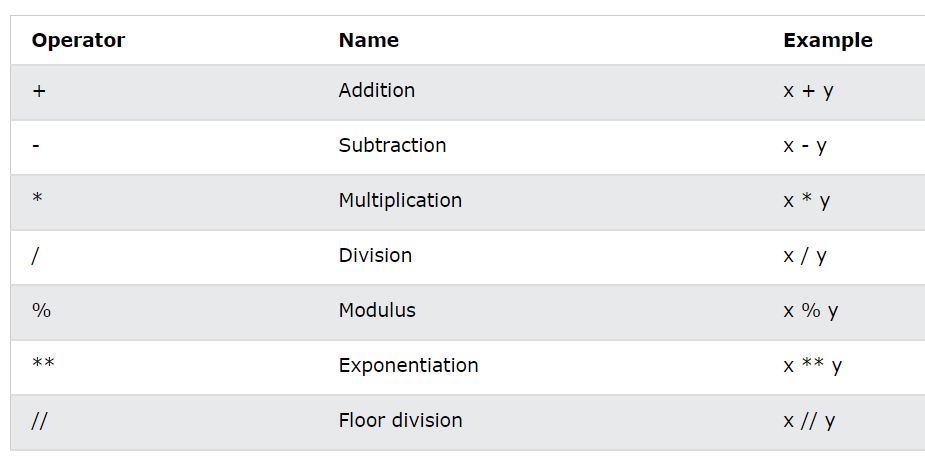
\includegraphics{assets/python.assets/bild1.png}
\caption{bild1}
\end{figure}

\hypertarget{vergleichsoperatoren}{%
\subsection{Vergleichsoperatoren}\label{vergleichsoperatoren}}

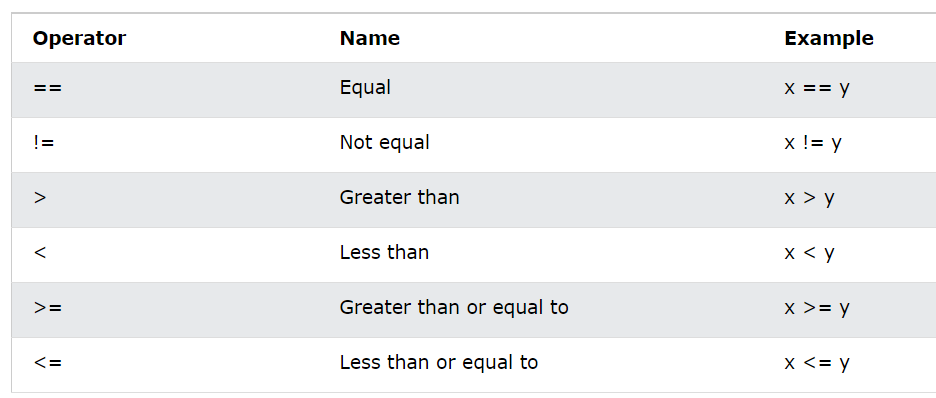
\includegraphics{assets/python.assets/image (187).png}

\hypertarget{logische-operatoren}{%
\subsection{Logische Operatoren}\label{logische-operatoren}}

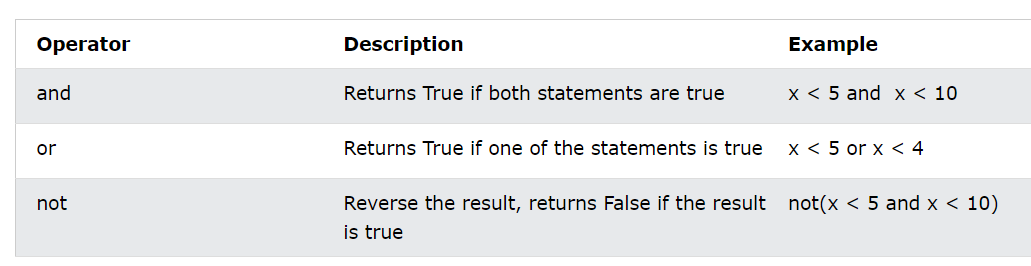
\includegraphics{assets/python.assets/image (188).png}

\hypertarget{datentypen-in-der-uxfcbersicht}{%
\section{Datentypen in der Übersicht}\label{datentypen-in-der-uxfcbersicht}}

Nachfolgendes Programmstück beschreibt exemplarisch die nun bekannten Datentypen. Mit \texttt{type()} kann man sich den Datentyp einer Variable ausgeben lassen (oft hilfreich!)

\begin{Shaded}
\begin{Highlighting}[]
\NormalTok{x }\OperatorTok{=} \DecValTok{1}\OperatorTok{;} 
\BuiltInTok{print}\NormalTok{( }\SpecialStringTok{f"1 : }\SpecialCharTok{\{}\BuiltInTok{type}\NormalTok{(x)}\SpecialCharTok{\}}\SpecialStringTok{"}\NormalTok{)}

\NormalTok{x }\OperatorTok{=} \FloatTok{1.1}\OperatorTok{;} 
\BuiltInTok{print}\NormalTok{( }\SpecialStringTok{f"1.1 : }\SpecialCharTok{\{}\BuiltInTok{type}\NormalTok{(x)}\SpecialCharTok{\}}\SpecialStringTok{"}\NormalTok{)}

\NormalTok{x }\OperatorTok{=} \DecValTok{4}\OperatorTok{/}\DecValTok{2}\OperatorTok{;} 
\BuiltInTok{print}\NormalTok{( }\SpecialStringTok{f"4/2 : }\SpecialCharTok{\{}\BuiltInTok{type}\NormalTok{(x)}\SpecialCharTok{\}}\SpecialStringTok{"}\NormalTok{)}

\NormalTok{x }\OperatorTok{=} \StringTok{\textquotesingle{}String\textquotesingle{}}\OperatorTok{;} 
\BuiltInTok{print}\NormalTok{( }\SpecialStringTok{f"\textquotesingle{}String\textquotesingle{} : }\SpecialCharTok{\{}\BuiltInTok{type}\NormalTok{(x)}\SpecialCharTok{\}}\SpecialStringTok{"}\NormalTok{)}

\NormalTok{x }\OperatorTok{=}\NormalTok{ [}\DecValTok{1}\NormalTok{,}\DecValTok{2}\NormalTok{,}\DecValTok{4}\NormalTok{]}\OperatorTok{;} 
\BuiltInTok{print}\NormalTok{( }\SpecialStringTok{f"[1,2,3] : }\SpecialCharTok{\{}\BuiltInTok{type}\NormalTok{(x)}\SpecialCharTok{\}}\SpecialStringTok{"}\NormalTok{)}

\NormalTok{x }\OperatorTok{=}\NormalTok{ (}\DecValTok{1}\NormalTok{,}\DecValTok{2}\NormalTok{)}\OperatorTok{;}
\BuiltInTok{print}\NormalTok{( }\SpecialStringTok{f"(1,2) : }\SpecialCharTok{\{}\BuiltInTok{type}\NormalTok{(x)}\SpecialCharTok{\}}\SpecialStringTok{"}\NormalTok{)}

\NormalTok{x }\OperatorTok{=} \DecValTok{1} \OperatorTok{\textless{}} \OperatorTok{{-}}\DecValTok{3}
\BuiltInTok{print}\NormalTok{( }\SpecialStringTok{f"False : }\SpecialCharTok{\{}\BuiltInTok{type}\NormalTok{(x)}\SpecialCharTok{\}}\SpecialStringTok{"}\NormalTok{)}
\end{Highlighting}
\end{Shaded}

\hypertarget{zusammenfassung}{%
\subsection{Zusammenfassung}\label{zusammenfassung}}

\begin{longtable}[]{@{}lll@{}}
\toprule
Eingebauter Datentyp & Kürzel & Beispiele \\
\midrule
\endhead
Text (Strings) & str & \texttt{x\ =\ "Haw-Landshut"} \\
Zahlen (Numerisch) & int, float & \texttt{x\ =\ 1} oder \texttt{x\ =\ 1.1} \\
Listen (Arrays) & list & \texttt{x\ =\ {[}1,2,3{]}} \\
Tupel & tuple & \texttt{x\ =\ (1,2)} \\
Wahrheitswerte & bool & \texttt{x\ =\ (1\ \textless{}\ 3)} \\
\bottomrule
\end{longtable}

\hypertarget{daten}{%
\chapter{Daten}\label{daten}}

\hypertarget{elementare-datentypen}{%
\section{Elementare Datentypen}\label{elementare-datentypen}}

Daten\footnote{sing. Datum} sind Ergebnisse von Beobachtungen, Messungen oder Berechnungen, die in einer bestimmten Form notiert, also aufgeschrieben sind. Häufig sprechen wir auch von \emph{Werten}, statt von Daten. Ein Werte kann zum Beispiel die Zahl \(27\) oder die Note ``\emph{sehr gut}'' sein. Offensichtlich gehören beide Werte zu verschiedene Typen von Werten, den sogenannten Datentypen. Wir beschäftigen uns mit den Datentypen \emph{Zahlen}, \emph{Text} und \emph{Boolean}

\hypertarget{zahlen}{%
\paragraph{Zahlen}\label{zahlen}}

Werte dieses Datentyps sind z.B. \(1\), \(-1\), \(1.7\) oder \(1/3\). Wie sie wissen, lässt sich die Menge der Zahlen noch weiter einteilen in natürliche Zahlen und reelle Zahlen (und noch ein paar mehr, die aber vorest nicht gebraucht werden. Wir verwenden die Symbole \(\mathbb{N}\) für die natürlichen Zahlen und \(\mathbb{R}\) für die reellen Zahlen.

Wir notieren Zahlen wie üblich und verwenden in der Dezimalnotation den Punkt als Trennsymbol.

\hypertarget{text}{%
\paragraph{Text}\label{text}}

Werte dieses Datentyps sind zum Beispiel ``Baum'', ``Hans Huber'' oder ``sehr gut''. Zeichenketten beginnen und enden mit einem Anführungszeichen. In der Regel macht uns diese Notationen keine Probleme - manchmal wird es trotzdem ungemütlich: Kann eine Zeichenkette ein Anführungszeichen enthalten? Gibt es einen Unterschied zwischen der Zahl 123 und der Zeichenkette ``123''? Wir vertiefen das hier nicht, sondern gehen die Fragen an, sobald sie uns begegnen.

\hypertarget{logischer-datentyp-boolean}{%
\paragraph{Logischer Datentyp (Boolean)}\label{logischer-datentyp-boolean}}

Dieser Datentyp umfasst nur zwei Werte, die sogenannten Wahrheitswerte. Wir werden in diesem Text die Notation \emph{True} und \emph{False} verwenden.

Wir nennen diese Datentypen ``elementar'', weil uns eine weitere Aufteilung nicht sinnvoll erscheint. Der Begriff ``elementar'' ist nicht ganz korrekt, weil z.B. die Zahl \(123\) ja eine Folge von Ziffern und die Zeichenkette ``Baum'' eine Folge von Buchstaben ist. Elementar wäre also eher der Datentyp \emph{Ziffer} oder \emph{Buchstabe}, als der Datentyp \emph{Zahl} oder \emph{Text}. Auch über diese begriffliche Ruppigkeit sehen wir zu Beginn hinweg. In der Programmierung werden sie aber eine Rolle spielen.

Stellen sie sich jeden Datentyp als Menge vor. Die Elemente der Menge sind die zulässigen Werte des Datentyps. Offensichtlich ist besitzt die Menge der Zahlen oder Texte unendlich viele Elemente, während der Logische Datentyp nur zwei Werte kennt.

\hypertarget{der-iris-datensatz}{%
\section{Der Iris-Datensatz}\label{der-iris-datensatz}}

Der Iris-Datensatz enthält Messungen von jeweils 50 Blüten zu drei verschiedenen Lilien-Arten (setosa, versicolor, virginica)

\begin{figure}
\centering
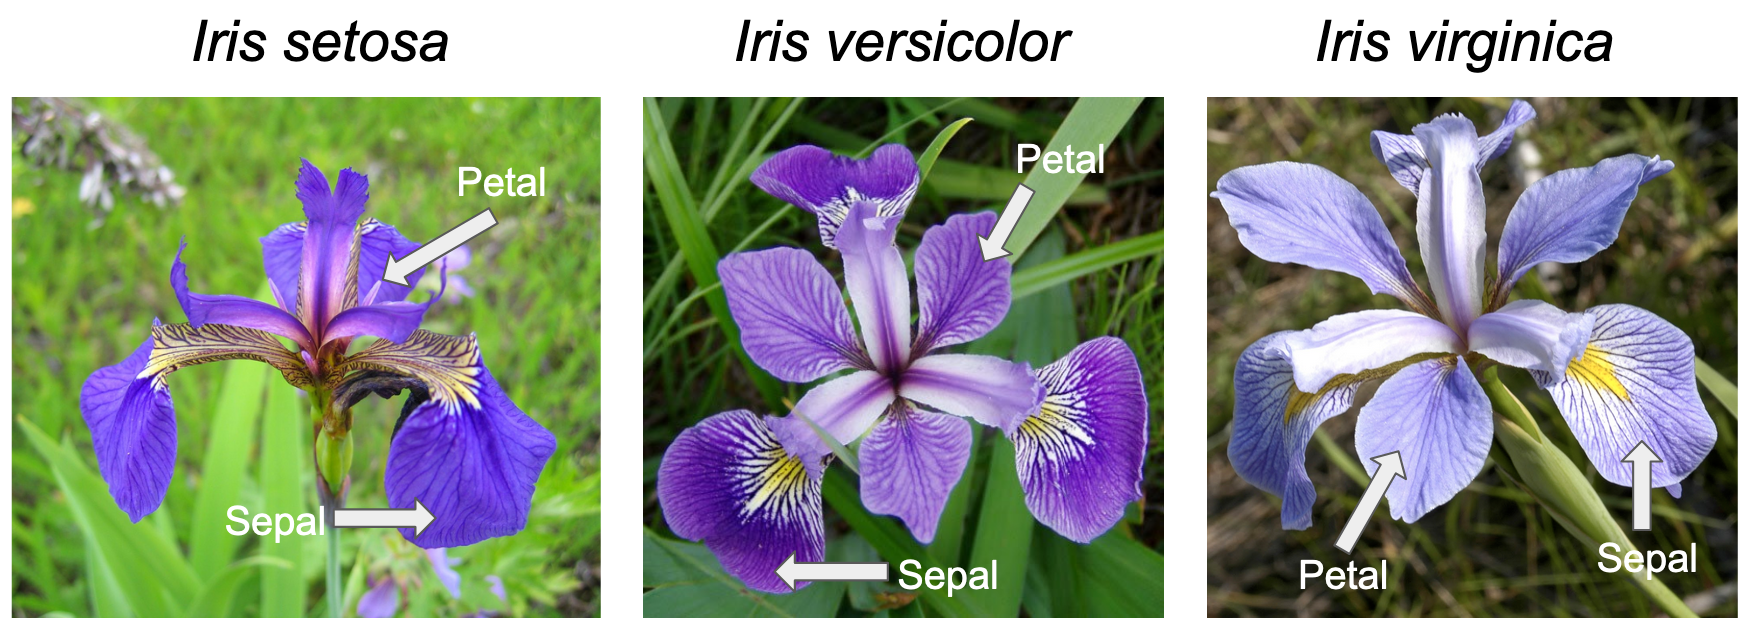
\includegraphics[width=1\textwidth,height=\textheight]{assets/daten.assets/Download.png}
\caption{Download}
\end{figure}

Gemessen werden pro \href{https://de.wikipedia.org/wiki/Bl\%C3\%BCte}{Blüte}in cm 

\begin{itemize}
\tightlist
\item
  die Länge und Breite des Kronblattes (Petalum, petal) sowie 
\item
  die Länge und Breite des Kelchblattes (Sepalum, sepal)
\end{itemize}

\begin{figure}
\centering
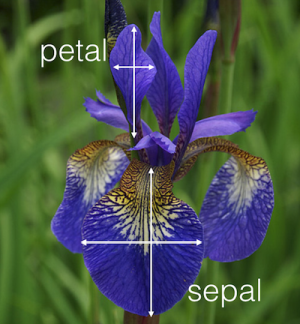
\includegraphics{assets/daten.assets/image_messung-16426070933692.png}
\caption{image (190)}
\end{figure}

\hypertarget{datensatz}{%
\subsection{Datensatz}\label{datensatz}}

Folgender - in der Community wohlbekannter - Datensatz liegt uns vor (Sie finden die Daten \href{https://syncandshare.lrz.de/getlink/fi89kxTJ5yLRaW5mnpyrofVK/Iris_p.xlsx}{hier}).

\begin{figure}
\centering
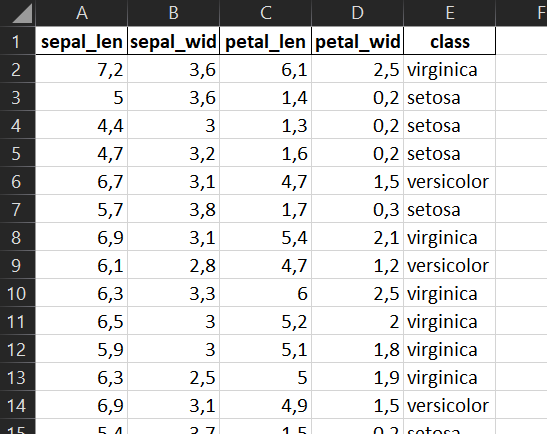
\includegraphics{assets/daten.assets/image-20211209101425856-16426070878651.png}
\caption{Iris-Datensatz}
\end{figure}

\hypertarget{datentypen-1}{%
\section{Datentypen}\label{datentypen-1}}

\hypertarget{elementare-datentypen-1}{%
\subsection{Elementare Datentypen}\label{elementare-datentypen-1}}

\hypertarget{zahlen-1}{%
\subsubsection{Zahlen}\label{zahlen-1}}

\hypertarget{strings}{%
\subsubsection{Strings}\label{strings}}

\hypertarget{logische-werte}{%
\subsubsection{Logische Werte}\label{logische-werte}}

\hypertarget{elementare-datentypen-in-python}{%
\subsubsection{Elementare Datentypen in Python}\label{elementare-datentypen-in-python}}

\hypertarget{komplexe-datentypen}{%
\subsection{Komplexe Datentypen}\label{komplexe-datentypen}}

\hypertarget{datum}{%
\subsubsection{Datum}\label{datum}}

\hypertarget{uhrzeit}{%
\subsubsection{Uhrzeit}\label{uhrzeit}}

\hypertarget{bilder}{%
\subsubsection{Bilder}\label{bilder}}

\hypertarget{komplexe-datentypen-in-python}{%
\subsubsection{Komplexe Datentypen in Python}\label{komplexe-datentypen-in-python}}

\hypertarget{skalenniveaus}{%
\section{Skalenniveaus}\label{skalenniveaus}}

\hypertarget{uxfcberblick}{%
\subsection{Überblick}\label{uxfcberblick}}

\begin{longtable}[]{@{}
  >{\raggedright\arraybackslash}p{(\columnwidth - 8\tabcolsep) * \real{0.0563}}
  >{\raggedright\arraybackslash}p{(\columnwidth - 8\tabcolsep) * \real{0.0915}}
  >{\raggedright\arraybackslash}p{(\columnwidth - 8\tabcolsep) * \real{0.4225}}
  >{\raggedright\arraybackslash}p{(\columnwidth - 8\tabcolsep) * \real{0.1268}}
  >{\raggedright\arraybackslash}p{(\columnwidth - 8\tabcolsep) * \real{0.3028}}@{}}
\toprule
\begin{minipage}[b]{\linewidth}\raggedright
Scale
\end{minipage} & \begin{minipage}[b]{\linewidth}\raggedright
Operations
\end{minipage} & \begin{minipage}[b]{\linewidth}\raggedright
Description
\end{minipage} & \begin{minipage}[b]{\linewidth}\raggedright
Statistics
\end{minipage} & \begin{minipage}[b]{\linewidth}\raggedright
Example
\end{minipage} \\
\midrule
\endhead
Nominal & \(=, \neq\) & values have no natural order; they describe unordered categories & Mode (Modus) & München, Hamburg, Essen \\
Ordinal & \(<, >\) & values have a defined order; difference of values is undefined or has no clear or meaningful definition & Median & Schulnoten, Tabellenplatz in der Bundesliga \\
Interval & \(+,-\) & differences of values have the same meaning; adding provides useful results; zero point is not naturally/globally defined & Mean & Temperatur \\
Ratio & \(\cdot , /\) & zero point is naturally defined & (Generalized) Mean & Alter \\
\bottomrule
\end{longtable}

Bemerkungen:

\begin{enumerate}
\def\labelenumi{\arabic{enumi}.}
\item
  Skalenniveaus sind nicht immer klar zuzuordnen.
\item
  Auf nominalen Datenskalen lassen sich stets \emph{künstliche Ordnungen} (und damit ordinale Datenskalen) definieren.
\item
  Bilden sie keine Mittelwerte auf Daten mit ordinalen Datenskalen!
\item
  Nominale und ordinale Datenskalen heißen auch \emph{kategorisch} oder \emph{qualitativ}.
\item
  Intervall und Ratio-Datenskalen heißen auch \emph{metrisch}.
\end{enumerate}

Ergänzend: \href{https://www.statistikpsychologie.de/skalenniveaus/}{Die fünf Skalenniveaus: Einfach und verständlich erklärt (statistikpsychologie.de)}

\hypertarget{skalenniveaus-im-iris-datensatz}{%
\subsection{Skalenniveaus im Iris-Datensatz}\label{skalenniveaus-im-iris-datensatz}}

\begin{figure}
\centering
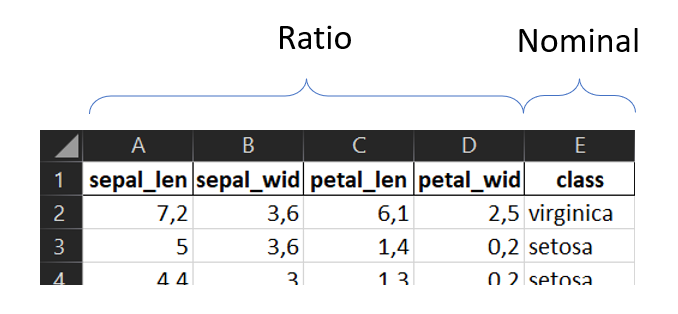
\includegraphics{assets/daten.assets/image-20211209145313372.png}
\caption{Skalenniveaus bei Iris}
\end{figure}

\hypertarget{von-nominal-zu-ordinal}{%
\paragraph{Von Nominal zu Ordinal}\label{von-nominal-zu-ordinal}}

Wir werden später folgende eindeutige Zuordnung treffen:

\begin{longtable}[]{@{}cc@{}}
\toprule
Nominaler Wert & Ordinaler Wert \\
\midrule
\endhead
setosa & 0 \\
versicolor & 1 \\
virginica & 2 \\
\bottomrule
\end{longtable}

\hypertarget{part-latex-part}{%
\part*{Latex Part}\label{part-latex-part}}
\addcontentsline{toc}{part}{Latex Part}

\hypertarget{chapter}{%
\chapter{Chapter}\label{chapter}}

\hypertarget{latex-section-h2}{%
\section{Latex Section (H2)}\label{latex-section-h2}}

Ich habe mich bemüht, zahlreiche Übungsbeispiele und Youtube-Videos einzubauen. Viele Themen lassen sich so besser darstellen. Sofern es Medien im Netz gibt,

Parskip!! die die Sachverhalte gut darstellen, werde ich entsprechenden Links einbauen. Der Autor muss ja nicht der Meinung sein, alles besser zu können. Gleichwohl darf dadurch der rote Faden nicht verl

\hypertarget{latex-subsection-h3}{%
\subsection{Latex Subsection (H3)}\label{latex-subsection-h3}}

Ich habe mich bemüht, zahlreiche Übungsbeispiele und Youtube-Videos einzubauen. Viele Themen lassen sich so besser darstellen. Sofern es Medien im Netz gibt, die die Sachverhalte gut darstellen, werde ich entsprechenden Links einbauen. Der Autor muss ja nicht der Meinung sein, alles besser zu können. Gleichwohl darf dadurch der rote Faden nicht verl

\hypertarget{latex-subsubsection-h4}{%
\subsubsection{Latex SubSubSection (H4)}\label{latex-subsubsection-h4}}

Ich habe mich bemüht, zahlreiche Übungsbeispiele und Youtube-Videos einzubauen. Viele Themen lassen sich so besser darstellen. Sofern es Medien im Netz gibt, die die Sachverhalte gut darstellen, werde ich entsprechenden Links einbauen. Der Autor muss ja nicht der Meinung sein, alles besser zu können. Gleichwohl darf dadurch der rote Faden nicht verl

\hypertarget{latex-paragraph-h5}{%
\paragraph{Latex Paragraph (H5)}\label{latex-paragraph-h5}}

Ich habe mich bemüht, zahlreiche Übungsbeispiele und Youtube-Videos einzubauen. Viele Themen lassen sich so besser darstellen. Sofern es Medien im Netz gibt, die die Sachverhalte gut darstellen, werde ich entsprechenden Links einbauen. Der Autor muss ja nicht der Meinung sein, alles besser zu können. Gleichwohl darf dadurch der rote Faden nicht verl

  \bibliography{book.bib,packages.bib}

\end{document}
